% !Mode:: "TeX:UTF-8"

% !TEX root = ../main.tex

\chapter{基于属性的凭证}[Attribute-Based Credentials]

基于属性的凭证是一种特殊的凭证系统。
在一个凭证系统中,通常有凭证发行机构、用户及验证者这三类角色。
用户可以从凭证发行机构处获取有效的凭证,验证者就可以通过校验用户凭证的真实性从而完成对用户的证明。
最常见的凭证就是用户的身份证。
在日常生活中,我们可以从派出所申请到有效的个人身份证。
当需要进行一些与验证身份有关的操作时,如在火车站买票,我们就可以通过出示身份证的方式来验证与身份有关的信息。

那么什么是基于属性的凭证呢?首先需要解释一下属性的概念。
一个人的身高、年龄、身体状况、学历等信息都可以看做这个人的属性信息。
因此,我们可以将身份看做是一组属性的集合。
图3-1表示的是Alice在不同场景下表现出的各个属性,而且这些属性都是直接与Alice的身份相关联的。

\begin{figure}[h]
\centering
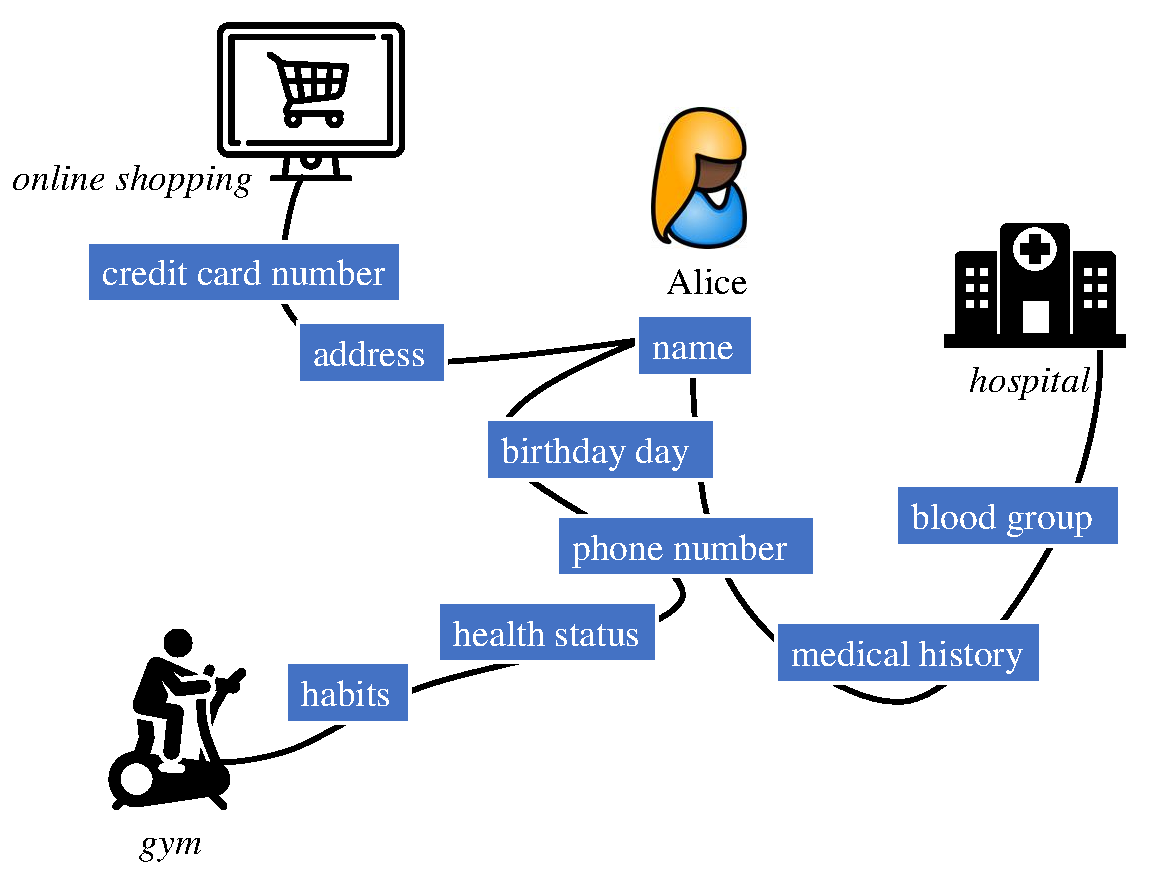
\includegraphics[width = 0.8\textwidth]{1-1}
\caption{Alice在不同场景下出示的属性信息}
\end{figure}

传统的凭证由于直接将属性信息与真实身份相关联,这样做会给Alice带来许多安全隐患。
比如Alice在去医院看病的过程中,医院就会得知Alice的血型、年龄及过往病史等一系列的信息。
这些信息都是直接跟Alice的身份挂钩,且大部分都是属于隐私的内容。
假如医院的数据库遭到攻击或医院直接出售这些信息,用户的个人信息安全将会面临巨大的威胁。

基于属性的凭证的作用是切断用户的属性与用户真实身份的关联,这种性质也被称为不可关联性(Unlinkability)。
因此在获取凭证的时候,用户需要的是获取对某个属性的凭证;在验证的过程中,用户只需提供必要属性的凭证即可,并且在整个验证的过程中,用户始终保持着匿名的状态。

\section{发展历程}[History]

基于属性的凭证的概念是从匿名凭证发展而来,而匿名凭证的思想最早是由Chaum\cite{chaum1985security}于1985年提出的,他主要围绕着如何在匿名的情况下完成交易提出了自己的一系列设想。
在这之后,Chaum与Evertse于1986年提出了一个解决方案\cite{chaum1986secure},这个方案需要有一个半诚实的(Semi-Honest)第三方机构\cite{张严2012匿名凭证方案研究进展,camenisch2001efficient},所谓的半诚实机构意味着它可以按照规则执行协议,也不会篡改执行的数据,但可以分析这些数据。这个方案由于可行性比较差,离实际应用还有一定距离。
经历了十多年的探索,同时也随着对数字签名,零知识证明等研究的不断深入,Camenisch和Lysyanskaya于2001年正式提出了第一个可行的匿名凭证方案\cite{camenisch2001efficient},这也是匿名凭证的概念第一次出现并被正式定义。
这个方案实现了包括假名生成,凭证的生成及凭证的展示等完整的协议,同时他们也对该方案的不可伪造性,匿名性,不可关联性及可行性等基本特性给出了完整的证明。
另外,他们在此基础上设计了一个扩展方案,这个扩展版的方案还满足了凭证不可出借及可撤销等与实际应用场景相关的特性。
作为第一个可行方案,此方案的安全性是基于强RSA假设和离散对数假设。

这个方案在构造上很大程度上受到假名系统(Pseudonym System)\cite{chen1996access,lysyanskaya1999pseudonym}的影响,也就是说,用户在请求凭证之前,需要从凭证发行者处获取假名,然后再使用假名的方式进行交互。
自第一个可行方案出现以后,关于匿名凭证的研究开始迈入新的篇章。
紧接着在2002年,Camenisch与Herreweghen给出了这一方案的具体实现,也就是Idemix系统\cite{camenisch2002design}。
同一时期,Brands基于盲签名的方法提出了一些有关匿名验证的思想\cite{brands1999rethinking},并在创建了Credentica公司之后基于此思想构建了一个匿名凭证系统U-Prove。
该系统随着2008年Credentica公司被微软收购由微软继续进行研发\cite{paquin2011u},已经成为最具代表性的匿名凭证系统之一。

匿名凭证系统的核心部分很大程度上依赖于数字签名,2001年的匿名凭证方案主要使用传统的RSA签名方案。
由于双线性映射的出现推动了数字签名的发展,伴随着许多基于双线性映射的签名方案的出现\cite{boneh2001short,camenisch2004signature,okamoto2006efficient},一些新的匿名凭证的方案构造也涌现出来。
基于双线性对的数字签名构造一般比较简洁,而且在同等安全条件下,签名长度相对RSA来说要短得多,如果用于匿名凭证的构造中会大大提高整个系统的效率。

2004年Camenisch和Lysyanskaya设计了一个基于双线性对的签名方案,并基于此签名方案提出了一个匿名凭证方案\cite{camenisch2004signature}。
在这个签名方案中,签名者可以在不知道签名内容$m$的情况下完成对$m$的签名。
更准确的说,签名者只知道$m$的承诺值$m'=\mathsf{Com}(m,r)$的情况下,生成对$m$的合法签名$\sigma$。
由于承诺机制满足隐藏和绑定这两个性质,在没有公开$r$的情况下,签名者无法获知所需签名的内容。
因此,这种签名方案能够用在匿名凭证系统的发行凭证这一过程中。
Camenisch和Lysyanskaya粗略地描述了利用此签名方案来构造匿名凭证系统的思路,构造出来的匿名凭证方案也没有提供可追踪性。
另一个基于此签名方案的是Blanton于2008年构造的一个匿名访问系统\cite{blanton2008online}。
这个系统可以看做匿名凭证系统的特殊情况,即把凭证发行机构与验证者合并起来看做一个服务提供商。
用户可以匿名地从服务商订阅服务,并以匿名的方式通过验证。
同年,Akagi,Manabe和Okamoto基于Okamoto提出的签名方案\cite{okamoto2006efficient}构造了一个包含完整的撤销机制的匿名凭证系统\cite{akagi2008efficient}。

由于普通的数字签名机制只能保证信息的完整性,并不能确保用户身份的匿名性。
因此在以上提到的匿名凭证系统中,为了保证匿名性,还使用了大量的零知识证明。
但是零知识证明需要多次的交互,且随着需要证明的内容增加,证明就变得越繁杂,这样就限制了匿名凭证系统的效率。
尽管我们可以使用Fiat-Shamir协议\cite{fiat1986prove}把一个交互式的零知识证明转换成一个非交互式的零知识证明,但是这种简单的转换无法用在双线性映射上\cite{张严2012匿名凭证方案研究进展},而且在安全性上需要基于随机预言机(Random Oracle)模型。

2008年,针对双线性映射上的非交互式零知识证明协议\cite{groth2008efficient}由Groth和Sahai提出,这种零知识证明协议(GS-Proof)具有一般性,因此能够很容易地应用到其他方案构造中。
自此之后,基于GS-Proof的匿名凭证系统方案也相继被提出\cite{belenkiy2008p,belenkiy2009randomizable}。
非交互式的证明方式为匿名凭证方案的构造带来了便利,更丰富了匿名凭证的应用场景。

在匿名凭证中比较重要的部分是对属性的签名,基于属性的凭证更能体现对属性的签名这一点。
自2012年之后,基于属性的凭证的概念开始替代了之前匿名凭证的称谓\cite{sabouri2012attribute},比如ABC4Trust这个项目中的ABC就是基于属性的凭证的英文缩写。
现在对基于属性的凭证的研究变得越来越细致,大多是针对特定的场景下设计可行的协议或针对某一个具体的性质进行改进。
比如有利用累加器(Accumulator)的方法来实现凭证撤销问题\cite{camenisch2009accumulator},或构建一个去中心化的基于属性的凭证系统\cite{garman2014decentralized},或利用结构保护的签名(Structure-Preserving Signature)来构造长度固定的凭证\cite{fuchsbauer2018structure},等等。

\section{基本结构及性质}[Construction]

在前面的介绍中,我们知道数字签名和零知识证明在基于属性的凭证方案的构造上起到了很关键的作用。
一般来说,凭证系统中的主要参与者可以分为用户(Users),凭证发行机构(Issuer)及验证者(Verifiers)这三类。
用户拥有者许多的属性,他们可以通过向凭证发行机构发起请求,以获取相关的属性凭证。
在获得相应的凭证之后,就可以通过匿名的方式提供相应的凭证给验证者,当通过验证后,用户就可以拥有获取相关服务的权限。
因此验证者有时也被称做服务提供者(Service Providers),三者之间的交互过程如图3-2所示。

\begin{figure}[h]
\centering
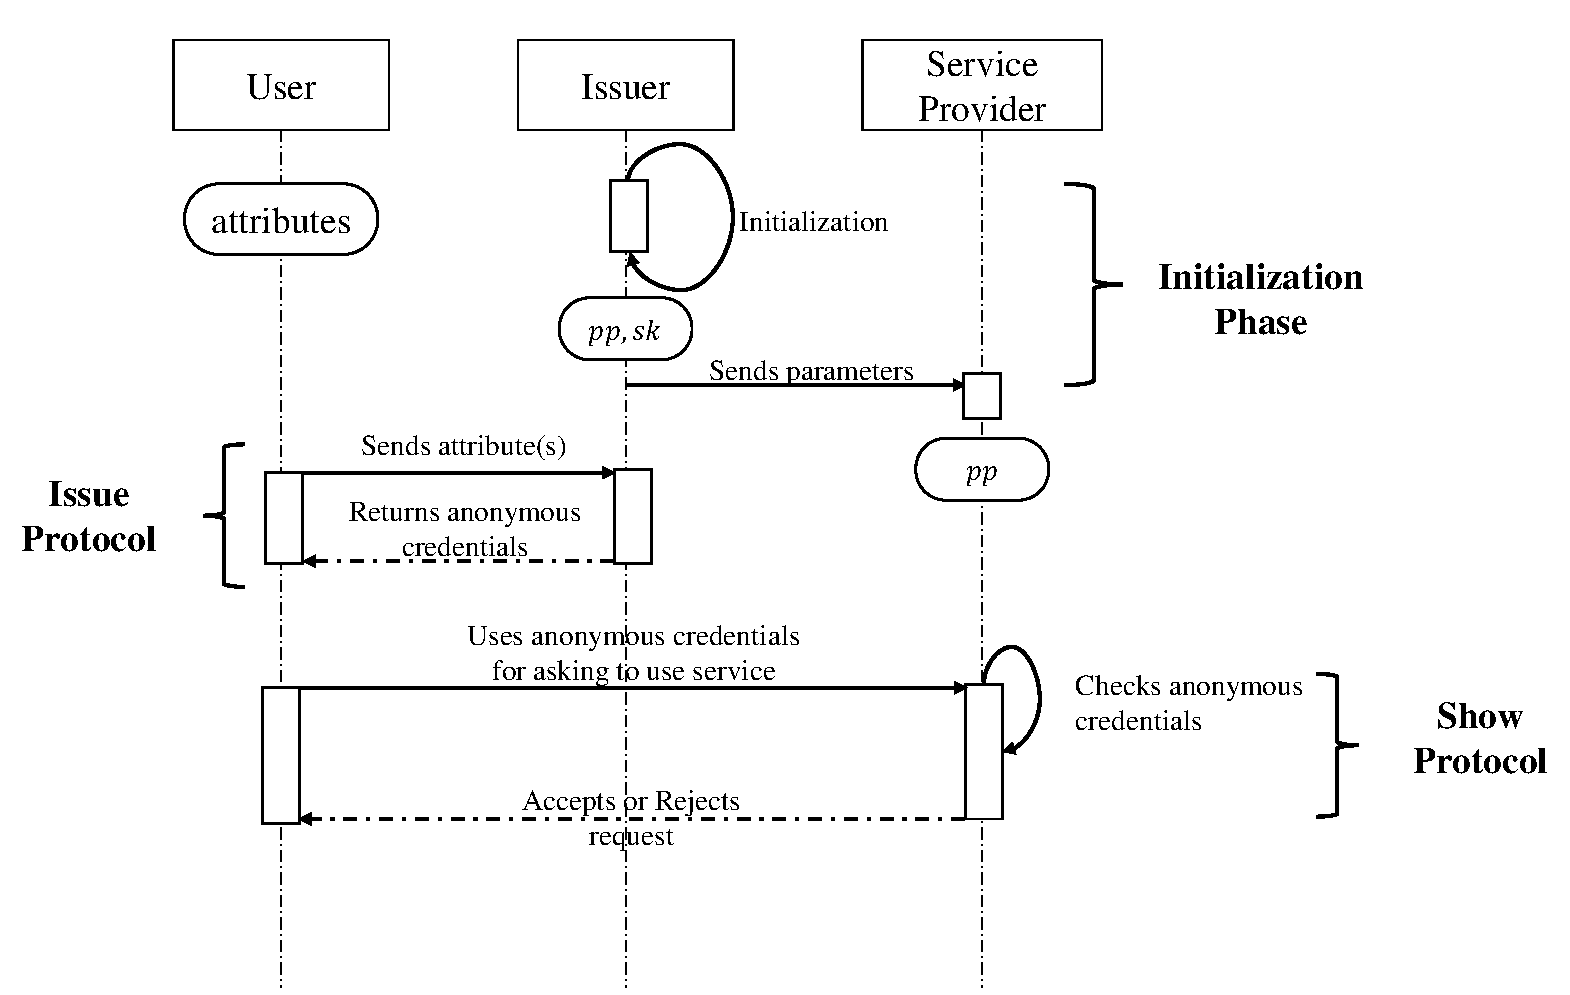
\includegraphics[width = 1\textwidth]{1-2}
\caption{基于属性的凭证系统中各角色交互的序列图}
\end{figure}

为了方便说明,下面我们分别用$\mathcal{U}$、$\mathcal{I}$和$\mathcal{V}$来表示用户,发行机构和验证者。
从图中我们可以看出,在一个基于属性的凭证系统中,主要包含初始化,发行凭证和使用凭证这三个阶段。
而要构造这样一个系统,关键在于如何实现发行凭证和出示凭证这两个协议。
初始化的过程一般是由$\mathcal{I}$来完成,一般在输入安全参数$\kappa$之后,得到系统输出的公共参数$pp$及私钥$sk$。
$\mathcal{I}$需要把$sk$保管起来,并将$pp$直接公开。$pp$一般包含系统的公钥及一些必要的参数,如在基于双线性映射的方案中,$pp$就包含$\mathbb{G}_1$,$\mathbb{G}_T$等信息。
$\mathcal{U}$在请求凭证之前,需要将自己的属性信息发送给$\mathcal{I}$。
当这些属性通过验证之后,$\mathcal{I}$可以使用$sk$对属性进行签名,并返回相应的基于属性的凭证。
在一些特殊情况下,$\mathcal{U}$不是直接把属性信息传递给$\mathcal{I}$,而是利用承诺机制对属性或一部分属性信息进行承诺,并将承诺结果发送给$\mathcal{I}$。
$\mathcal{U}$就可以利用这个凭证完成对属性的证明,$\mathcal{V}$利用之前收到的$pp$,就可以对凭证的真实性进行验证。
为了确保$\mathcal{U}$的身份不被泄漏,这里一般使用零知识证明的方式完成整个验证过程。

由此可知,在一个基于属性的凭证系统中,需要满足两个基本的性质,即可验证性(Authenticity)和匿名性(Anonymity)。

\begin{itemize}
  \item 可验证性:用户只有在拥有合法的凭证的情况下才能通过$\mathcal{V}$的验证。合法的凭证指的是此凭证是由$\mathcal{U}$从$\mathcal{I}$处获取且凭证没有被撤销。
  从另一个角度来说,满足可验证性即表示也满足不可伪造性,即用户$\mathcal{U}$不能伪造出一个合法的凭证。可验证性是由$\mathcal{I}$所使用的签名算法保证的。
  \item 匿名性:也可以称为身份与属性的不可关联性,即在$\mathcal{V}$通过$\mathcal{U}$的验证后,$\mathcal{V}$除了知道$\mathcal{U}$拥有相应的属性信息之外,并不能知道用户的真实身份。这主要是利用零知识证明的方式来实现的,通过这种方式可以充分地保护用户隐私。
\end{itemize}

除了这两个基本的性质外,针对现实生活中的场景,我们往往还需要考虑下面这几个性质:

\begin{itemize}
  \item 凭证的不可关联性:$\mathcal{U}$使用不同的凭证与$\mathcal{V}$交互,对于$\mathcal{V}$来说,不能判断出这多个凭证来自同一个用户。
  \item 可追踪性: 可追踪性指的是在必要的情况下,凭证的使用者是可以被还原出来的。因此如果满足了可追踪性,那也意味着此凭证不是绝对匿名的。
  执行追踪的一般是凭证发行机构$\mathcal{I}$或一个可信的第三方组织$\mathcal{O}$。此外,$\mathcal{O}$还需要满足不能伪造凭证这一性质。
  \item 可撤销性: 撤销一般是在凭证到期了或凭证被恶意使用的情况下执行的。要实现可撤销性,一般需要先实现可追踪性。在实际的应用场景中,可撤销还是一个很必要的特性。
\end{itemize}

\section{相关实例}[Application]

在这一节我们主要介绍已有的匿名凭证实例,这些实例包括IdeMix、U-Prove和ABC4Trust。

\subsection{IdeMix}[idemix]

IdeMix\cite{camenisch2002design}是第一个完整地实现了凭证的签发协议,使用协议并且支持撤销的匿名凭证系统,它是由Camenisch和Herreweghen在2002年设计出来的。
理论上主要基于Camenisch与Lysyanskaya在2001年提出的第一个匿名凭证方案\cite{camenisch2001efficient},这个方案使用的是RSA密码体制,安全性依赖于大整数分解的困难性。

在这个系统中,主要的参与者还是用户$\mathcal{U}$,凭证发行机构$\mathcal{I}$和验证者$\mathcal{V}$。
其中包含两个基本协议,即生成协议(Generation Protocol)与出示协议(Show Protocol),这两个基本协议中又包含了许多子协议。

\begin{itemize}
  \item[1.] \textbf{生成协议:}主要包含假名生成协议与凭证生成协议。$\mathcal{U}$通过向$\mathcal{I}$发送请求,以获取假名。
  然后用户就可以使用假名从$\mathcal{I}$处获取相应的凭证。
  \item[2.] \textbf{出示协议:}此协议主要是$\mathcal{U}$向$\mathcal{V}$证明自己拥有某个凭证,从而获取使用$\mathcal{V}$所提供的服务的权限。
\end{itemize}

在匿名凭证系统中,拥有一个可信的$\mathcal{I}$是很重要的,因为$\mathcal{I}$会保存着用户假名与凭证的对应关系。
因此,用户在与$\mathcal{I}$请求凭证的时候,可以每次选择不同的假名,这样能避免凭证与真实身份之间的关联。
$\mathcal{V}$作为服务提供者,可以看作一个提供在线视频的网站,或一个在线购物商城。
利用此系统,用户就可以用匿名的形式获取相关在线服务。
IdeMix系统不仅可以支持线上的服务,也可以支持离线的服务,如在智能卡上的应用\cite{bichsel2009anonymous}。

\subsection{U-Prove}[uprove]

U-Prove是微软公司开发的匿名凭证系统,它主要基于公钥密码学,椭圆曲线和哈希函数。
系统中也存在用户$\mathcal{U}$,凭证发行者$\mathcal{I}$以及验证者$\mathcal{V}$这三类角色。
与IdeMix类似,U-Prove中也包含生成和出示这两个基本的协议,但细节有所不同。

\begin{itemize}
  \item[1.] \textbf{生成协议:} $\mathcal{U}$从$\mathcal{V}$处获取一个token。
  \item[2.] \textbf{出示协议:} $\mathcal{U}$使用token通过$\mathcal{V}$的验证。
\end{itemize}

这里的token就包含了用户的属性信息。
通过使用一些密码学的方法,可以保证token不被篡改。
在U-Porve中,发行者$\mathcal{I}$使用的是盲签名的方式,用户$\mathcal{U}$则采取零知识证明的方式与$\mathcal{V}$进行交互。
此系统很好地保证了token与用户身份的不可关联性,但是如果多次使用同一个token则会破坏此不可关联性。
因此用户在每次验证前都需要使用一个新的token,只有这样才能确保完全的不可关联。

\subsection{ABC4Trust}[abc]

\begin{figure}[h]
\centering
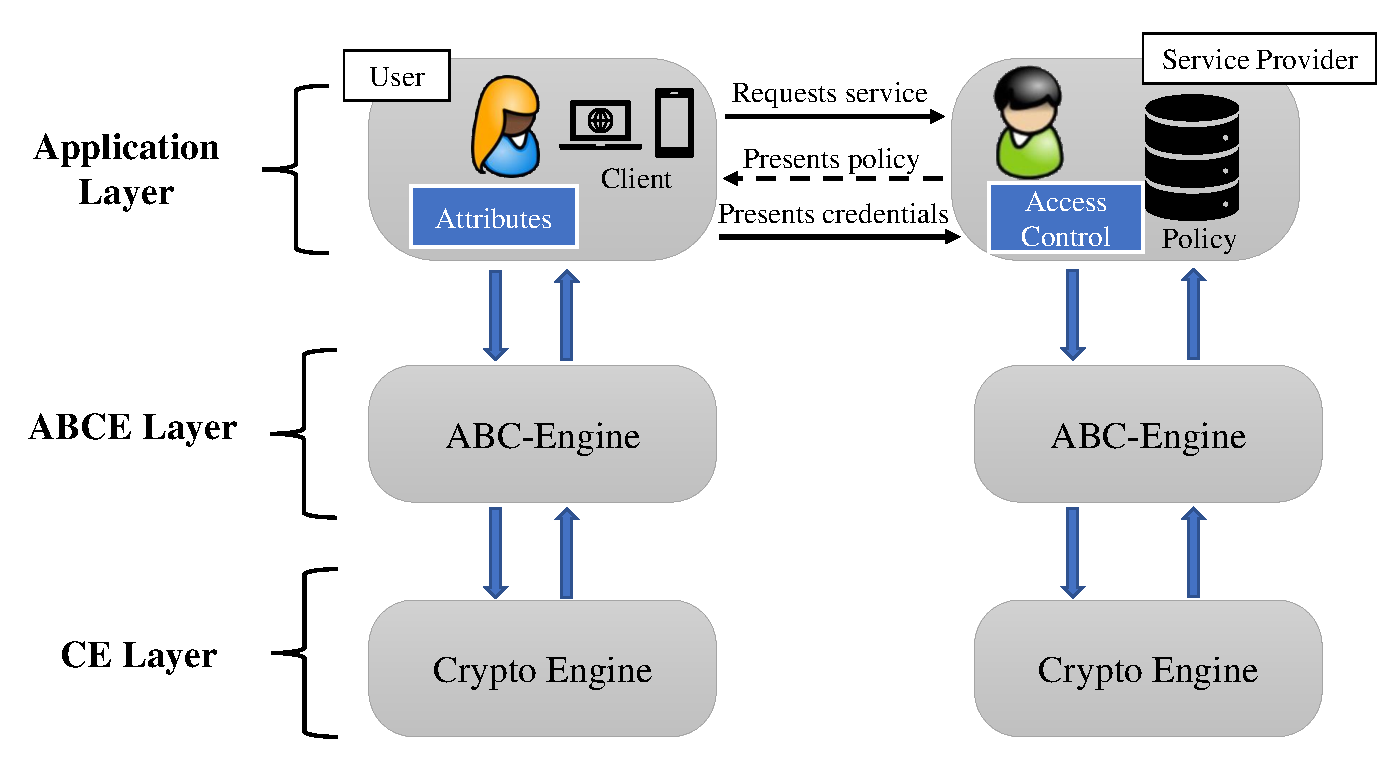
\includegraphics[width = 0.9\textwidth]{1-3}
\caption{ABC4Trust的基本结构}
\end{figure}

ABC4Trust,全称为Attribute-Based Credential for Trust,它是由欧盟资助的用来保护个人隐私的项目\cite{sabouri2012attribute}。
与前两个项目不同,ABC4Trust不仅关注在协议的设计,更多的是为基于属性的系统构建了一个完整的开发框架。
此项目为构建基于属性的凭证系统提供了一个完整的框架,它把用户$\mathcal{U}$与验证者$\mathcal{V}$之间交互的过程分成了三层,从上到下分别是应用层,ABC-Engine层和Crypto-Engine层。

正因为这种划分,我们可以在底层使用不同的密码学协议,层与层之间只需要提供相应的API接口即可。
ABC4Trust为基于属性的凭证系统的构造提供了一个比较规范的框架,这大大方便了开发者的对此类凭证系统的开发。

\section{本章小结}[Summary III]

在这一章,我们首先介绍了基于属性的凭证的发展历程,重点描述匿名凭证系统发展的几个阶段以及不同阶段的研究内容。
然后我们介绍了基于属性的凭证系统的基本结构及其需要满足的一些性质。
最后通过描述IdeMix,U-Prove和ABC4Trust这三个比较有代表性的现实生活中的实例,来说明匿名凭证系统的发展趋势。
其中IdeMix深受假名系统的影响,U-Prove利用了数字签名、承诺机制与零知识证明等方案,也是现在构建一个匿名凭证系统的常见做法。
ABC4Trust则着重于框架的设计,意在实现一套基于属性的凭证的标准。
通过对这几个实例的探讨,我们可以发现,随着对匿名凭证系统研究的深入,在构造方面逐步趋于规范化。
近年来,基于属性的凭证系统逐渐走向人们的生活中,在医疗、电子货币、电子身份证及物联网等方面都开始有了实际的应用\cite{neven2017privacy,viejo2019secure,de2018attribute}。